\documentclass[a4paper]{article}
\usepackage[italian]{babel}
\usepackage[italian]{isodate}  		% formato delle date in italiano
\usepackage{graphicx}				% gestione delle immagini
\usepackage{amsfonts}
\usepackage{booktabs}				% tabelle di qualità superiore
\usepackage{amsmath}				% pacchetto matematica
\usepackage{enumitem}				% gestione delle liste
\usepackage{pifont}					% pacchetto con elenchi carini
\usepackage[x11names]{xcolor}		% colori aggiuntivi
% Link ipertestuali per l'indice
\usepackage{xcolor}
\usepackage[linkcolor=black, citecolor=blue, urlcolor=cyan]{hyperref}
\hypersetup{
	colorlinks=true
}

%\usepackage{showframe}				% visualizzazione bordi
%\usepackage{showkeys}				% visualizzazione etichetta

\begin{document}
	\author{VR443470}
	\title{Reti di calcolatori}
	\date{\printdayoff\today}
	\maketitle
	
	\newpage
	
	% indice
	\tableofcontents
	
	\newpage
	
	%%%%%%%%%%%%%%%%
	% Introduzione %
	%%%%%%%%%%%%%%%%
	\section{Introduzione}
	
	\textbf{Internet} è una rete di calcolatori che interconnette miliardi di dispositivi di calcolo in tutto il mondo. Gli strumenti in una rete, per esempio cellulari o computer, vengono chiamati \textbf{host} (\emph{ospiti}) o \textbf{sistemi periferici} (\emph{end system}). Essi sono connessi tra di loro tramite una \textbf{rete di collegamenti} (\emph{communication link}) e \textbf{commutatori di pacchetti} (\emph{packet switch}). I collegamenti possono essere di vario tipo: cavi coassiali, fili di rame, fibre ottiche e onde elettromagnetiche. \newline
	Ogni collegamento detiene una sua \textbf{velocità di trasmissione} (\emph{transmission rate}), ovvero la velocità di trasmissione dei dati. L’\textbf{unità di misura} è il bit per secondo (bit/secondo, \emph{bps}).
	
	L’insieme delle informazioni, o dati, che vengono inviati o ricevuti prendono il nome di \textbf{pacchetto}. L’\textbf{obbiettivo} \underline{di un commutatore di pacchetti} è quello di ricevere un pacchetto che arriva da un collegamento in ingresso e di ritrasmetterlo su un collegamento d’uscita. I due \underline{principali commutatori} di internet sono: \emph{router} e i commutatori a livello di collegamento (\emph{link-layer switch}). La sequenza di collegamenti e di commutatori di pacchetto attraversata dal singolo pacchetto è nota come \textbf{percorso} o \textbf{cammino} (\emph{route} o \emph{path}).
	
	Quindi, in sintesi, le definizioni più rilevanti sono:
	
	\begin{itemize}
		\item[\ding{42}] \textcolor{Red3}{\textbf{Internet.}} Rete di calcolatori che interconnette i dispositivi di calcolo di tutto il mondo.
		
		\item[\ding{42}] \textcolor{Red3}{\textbf{Host (\emph{o} sistemi periferici).}} Strumenti in una rete, per esempio computer.
		
		\item[\ding{42}] \textcolor{Red3}{\textbf{Rete di collegamenti (\emph{communication link}) e commutatori di pacchetto (\emph{packet switch}).}} Collega vari \emph{host}, per esempio cavi coassiali o fili di rame.
		
		\item[\ding{42}] \textcolor{Red3}{\textbf{Velocità di trasmissione (\emph{transmission rate})}}. È la velocità di trasmissione dei dati e solitamente la sua \textbf{unità di misura} è il bit per secondo, cioè \emph{bps}.
		
		\item[\ding{42}] \textcolor{Red3}{\textbf{Pacchetto.}} Insieme delle informazioni che vengono inviate e ricevute.
		
		\item[\ding{42}] \textcolor{Red3}{\textbf{\underline{Obbiettivo}} commutatore di pacchetti.} Ricevere un pacchetto proveniente da un collegamento in ingresso e ritrasmetterlo su un collegamento d'uscita. Per esempio i \emph{router}.
		
		\item[\ding{42}] \textcolor{Red3}{\textbf{Percorso (\emph{route}) o cammino (\emph{path}).}} Sequenza di collegamenti e di commutatori di pacchetto attraversata dal singolo pacchetto.
	\end{itemize}

	\newpage
	
	%%%%%%%%%%%%%%%%%%%%%%%%%%%%%%%%%%%%%%%%%%%%%%%%%%%%%
	% ISP, TCP/IP, commutazione dei pacchetti e ritardi %
	%%%%%%%%%%%%%%%%%%%%%%%%%%%%%%%%%%%%%%%%%%%%%%%%%%%%%
	\section{ISP, TCP/IP, commutazione dei pacchetti e ritardi}
	
	\subsection{ISP}
	
	I sistemi periferici accedono ad Internet tramite un servizio chiamato \textbf{Internet Service Provider} (ISP). Con \textbf{provider} si intende un insieme di commutatori di pacchetto e di collegamenti. Gli \textbf{obbiettivi} degli ISP è fornire ai sistemi periferici svariati tipi di accesso alla rete, come quello residenziale a larga banda (e.g. DSL), quello in rete locale ad alta velocità, quello senza fili (\emph{wireless}) e in mobilità.
	
	\noindent
	Esistono \textbf{$3$ tipi} di livelli di ISP:
	
	\begin{description}
		\item{\textbf{Livello 1.}} \emph{Internazionale} (Telecom, TIM, ...);
		\item{\textbf{Livello 2.}} \emph{Nazionale} (Fastweb);
		\item{\textbf{Livello 3.}} \emph{Locale} (solitamente per professionisti).
	\end{description}

	Più è basso il livello, più gli ISP sono costituiti da \emph{router} ad alta velocità interconnessi tipicamente tramite fibra ottica.
	
	\subsection{TCP/IP}
	
	I sistemi periferici, i commutatori di pacchetto e altre parti di Internet fanno uso di \textbf{protocolli} che controllano l’invio e la ricezione di informazioni all’interno della rete. Esistono \textbf{due principali protocolli} Internet: \textbf{\emph{Transmission Control Protocol}} (TCP) e \textbf{\emph{Internet Protocol}} (IP). In particolare, l’IP specifica il formato dei pacchetti scambiati tra router e sistemi periferici. Generalmente ci si riferisce a questi due protocolli tramite il nome collettivo TCP/IP.
	
	\newpage
	
	\subsection{Commutazione dei pacchetti}
	
	Esistono due diversi approcci per spostare quantità di dati all’interno di una rete: la \textbf{commutazione di circuito} e la \textbf{commutazione di pacchetto}.
	
	\begin{center}
		\large \textcolor{Red3}{\textbf{Commutazione di circuito}}
	\end{center}
	
	Nella \textbf{commutazione di circuito} le risorse richieste lungo un percorso (buffer e velocità di trasmissione sui collegamenti) sono \textbf{riservate} per l'intera durata della sessione di comunicazione.
	
	\noindent
	\textcolor{Green4}{\textbf{Vantaggi:}}
	
	\begin{itemize}
		\item[\ding{51}] \textbf{Velocità costante} durante il collegamento poiché le risorse sono riservate e non condivise. Questo si traduce in un \textbf{ritardo contenuto}.
	\end{itemize}

	\noindent
	\textcolor{Red1}{\textbf{Svantaggi:}}
	
	\begin{itemize}
			\item[\ding{55}] \textbf{Spreco di risorse} poiché i circuiti sono inattivi durante i periodi di silenzio, ovvero nei periodi in cui non c’è comunicazione;
			
			\item[\ding{55}] \textbf{Complicazioni} nello stabilire circuiti e nel riservare larghezza di banda \emph{end-to-end}.
	\end{itemize}

	In questo contesto, i ritardi possono essere causati solamente per tre motivi: (1) a causa dell'instaurazione del circuito, (2) a causa della distanza tra sorgente e destinazione, (3) a causa della trasmissione vera e propria.
	
	\begin{center}
		\large \textcolor{Red3}{\textbf{Commutazione di pacchetto}}
	\end{center}

	Nella \textbf{commutazione di pacchetto} la sorgente divide i messaggi in parti più piccole, ovvero in \textbf{pacchetti} assegnando a ciascuno un'intestazione. I pacchetti viaggiano attraverso collegamenti e commutatori di pacchetto dalla sorgente alla destinazione.
	
	\noindent
	\textcolor{Green4}{\textbf{Vantaggi:}}
	
	\begin{itemize}
		\item[\ding{51}] \textbf{Ottimizzazione} delle risorse poiché c’è una condivisione di esse nei momenti di inattività.
	\end{itemize}
	
	\noindent
	\textcolor{Red1}{\textbf{Svantaggi:}}
	
	\begin{itemize}
		\item[\ding{55}] \textbf{Possibile perdita} di pacchetti nel caso in cui un buffer di un nodo sia saturo. Questo comporta un buffer overflow e una conseguente perdita;
		
		\item[\ding{55}] \textbf{Ritardo dovuto a \emph{store and forward} e numero di nodi intermedi.} A causa dello \emph{store and forward}, ogni nodo deve attendere di ricevere l'intero pacchetto prima di ritrasmetterlo. Inoltre, con l'aumentare dei nodi intermedi, il ritardo aumenta.\newline
		(approfondimento \href{https://it.wikipedia.org/wiki/Store_and_forward#:~:text=Nelle%20telecomunicazioni%2C%20lo%20store%20and,ritrasmesso%20nel%20collegamento%20in%20uscita}{\emph{store and forward}})
	\end{itemize}
	
	\newpage
	
	\subsection{Tipologie di ritardi}
	
	Esistono diverse tipologie di ritardo perché quando un pacchetto parte da un \emph{host} (sorgente), passa attraverso una serie di \emph{router} e conclude il viaggio in un altro \emph{host} (destinazione). Questo comporta un ritardo in ciascun nodo (\emph{host} o \emph{router}). I principali ritardi sono: \textbf{ritardo di elaborazione}, \textbf{ritardo di accodamento}, \textbf{ritardo di trasmissione} e \textbf{ritardo di propagazione}. L'insieme di questi ritardi è chiamato \textbf{ritardo totale di nodo} (\emph{nodal delay}).
	
	\begin{flushleft}
		\large \textcolor{Red3}{\textbf{Ritardo di elaborazione}}
	\end{flushleft}
	
	\noindent
	Il tempo richiesto per esaminare l’intestazione del pacchetto e per determinare dove dirigerlo fa parte del \textbf{ritardo di elaborazione} (\emph{processing delay}). Per dirigere si intende il tempo che impiega il \emph{router} a determinare la sua parte di uscita.
	
	\begin{flushleft}
		\large \textcolor{Red3}{\textbf{Ritardo di accodamento}}
	\end{flushleft}
	
	\noindent
	Una volta in coda, il pacchetto subisce un \textbf{ritardo di accodamento} (\emph{queuing delay}) mentre attende la trasmissione sul collegamento. La lunghezza di tale ritardo dipenderà dal numero di pacchetto precedentemente arrivati, accodati e in attesa di trasmissione sullo stesso collegamento. In altre parole, è il tempo speso nel \emph{buffer} prima che il pacchetto venga ritrasmesso.
	
	\begin{flushleft}
		\large \textcolor{Red3}{\textbf{Ritardo di trasmissione}}
	\end{flushleft}
	
	\noindent
	Data $L$ la lunghezza del pacchetto, in bit, e $R$ \emph{bps} la velocità di trasmissione del collegamento dal \emph{router} $A$ al \emph{router} $B$, il \textbf{ritardo di trasmissione} (\emph{transmission delay}) sarà $L\div R$. Questo è il tempo richiesto per trasmettere tutti i bit del pacchetto sul collegamento.\newline
	Più semplicemente, dipende dalla velocità di trasmissione e dalla dimensione del pacchetto ed è possibile sintetizzarlo con la formula:
	
	\begin{equation*}
		t_{\text{trasm}} = \dfrac{\text{dim\_pacchetto}}{\text{velocità\_trasmissione}}
	\end{equation*}
	
	\begin{flushleft}
	\large \textcolor{Red3}{\textbf{Ritardo di propagazione}}
	\end{flushleft}
	
	\noindent
	Una volta immesso sul collegamento, un bit deve propagarsi fino al \emph{router} B. Il tempo impiegato è il \textbf{ritardo di propagazione} (\emph{propagation delay}). In altre parole è il tempo impiegato per percorrere la distanza verso il \emph{router} successivo.
	
	\begin{flushleft}
		\large \textbf{Strumenti di misurazione}
	\end{flushleft}
	
	\noindent
	Esistono diversi \textbf{strumenti per misurare il ritardo}:
	
	\begin{itemize}
		\item \textbf{PING.} Dato un indirizzo di destinazione, il calcolatore manda una serie di messaggi e misura il tempo che intercorre tra l'invio e la ricezione della risposta, chiamato anche \emph{Rount Trip Time} (RTT).
		
		\item \textbf{TRACEROUTE.} Misura il \emph{Round Trip Time} tra la sorgente e \textbf{tutti} gli apparati di rete intermedi.
	\end{itemize}
	
	\newpage
	
	\subsection{Sintesi}
	
	\begin{itemize}[label=\ding{219}]
		\item \textbf{\emph{Internet Service Provider} (ISP).} Strumento utilizzato dai sistemi periferici per accedere ad Internet.
		
		\item \textbf{\emph{Provider}.} Insieme di commutatori di pacchetto e di collegamenti, solitamente è un'azienda che fornisce servizi.
		
		\item \textbf{\underline{Obbiettivi} ISP.} Fornire vari tipi di accesso alla rete ai dispositivi che si collegano (e.g. DSL, \emph{wireless}, ecc.).
		
		\item \textbf{\underline{Tipi} di ISP:}
			\begin{itemize}
				\item{\textbf{Livello 1.}} \emph{Internazionale} (Telecom, TIM, ...);
				\item{\textbf{Livello 2.}} \emph{Nazionale} (Fastweb);
				\item{\textbf{Livello 3.}} \emph{Locale} (solitamente per professionisti).
			\end{itemize}
		
		\item \textbf{Definizione TCP/IP.} Protocolli più famosi utilizzati dai sistemi periferici, i commutatori di pacchetto e altre parti di Internet. N.B. il protocollo IP specifica il formato dei pacchetti scambiati tra \emph{router} e sistemi periferici.
		
		\item \textbf{Definizione commutazione di circuito.}  Le risorse sono \underline{riservate} per l'intera comunicazione.
		
		\begin{enumerate}[label=\ding{43}]
			\item \textbf{\underline{Vantaggio} commutazione di circuito.} Velocità costante grazie ad un canale dedicato e quindi ritardo contenuto.
			
			\item \textbf{\underline{Svantaggio} commutazione di circuito.} Spreco di risorse in caso di silenzi durante la comunicazione.
			
			\item \textbf{\underline{Causa dei ritardi} nella commutazione di circuito.} I motivi possono essere tre:
			\begin{enumerate}[label=\Roman*]
				\item Instaurazione del circuito;
				\item Distanza tra sorgente e destinazione;
				\item Trasmissione vera e propria della comunicazione.
			\end{enumerate}
		\end{enumerate}
		
		\item \textbf{Definizione commutazione di pacchetto.} La sorgente divide i messaggi in parti più piccole chiamate \textbf{pacchetti}.
		
		\begin{enumerate}[label=\ding{43}]
			\item \textbf{\underline{Vantaggio} commutazione di pacchetto.} Ottimizzazione delle risorse poiché c'è una condivisione durante l'inattività.
			
			\item \textbf{\underline{Svantaggi} commutazione di circuito.} Eventuale perdita di pacchetti nel caso in cui un nodo intermedio abbia il \emph{buffer} saturo (generazione di \emph{buffer overflow}); ritardo causato da \emph{store and forward} poiché ogni pacchetto per essere inoltrato deve essere completamente trasmesso; all'aumentare dei nodi intermedi, il ritardo aumenta.
		\end{enumerate}
	
		\item \textbf{Ritardo di elaborazione (\emph{processing delay}).} Tempo impiegato dal \emph{router} per esaminare l'intestazione del pacchetto e determinare l'uscita.
		
		\item \textbf{Ritardo di accodamento (\emph{queuing delay}).} Tempo impiegato dal pacchetto all'interno della coda del buffer del \emph{router}.
		
		\item \textbf{Ritardo di trasmissione (\emph{transmission delay}).} Tempo che dipende dal rapporto tra la dimensione del pacchetto e la velocità di trasmissione.
		
		\item \textbf{Ritardo di propagazione (\emph{propagation delay}).} Tempo impiegato per percorrere la distanza verso il \emph{router} successivo.
		
		\item \textbf{Strumenti per la misurazione del ritardo.} I due strumenti sono ``PING'' e ``TRACEROUTE''. La differenza è che PING misura il RTT tra sorgente e destinazione, mentre il TRACEROUTE misura il RTT tra sorgente e \underline{ogni} nodo intermedio.
	\end{itemize}

	\newpage

	%%%%%%%%%%%%%%%%%%%%%%%%%%%%%%%%%%%%%%%%%%%%%%%%%%%%%%%%%%%%%%
	% Tecnica di load balancing, Throughput e collo di bottiglia %
	%%%%%%%%%%%%%%%%%%%%%%%%%%%%%%%%%%%%%%%%%%%%%%%%%%%%%%%%%%%%%%
	\section{Tecnica di load balancing, Throughput e collo di bottiglia}
	
	\subsection{Tecnica di load balancing}
	
	Nel momento in cui il \textbf{mittente} (sorgente) calcola il \textbf{percorso migliore} per inviare i suoi dati al destinatario, può accadere che \textbf{trovi due o più strade identiche}. Con quest'ultimo termine si intende che i percorsi con il costo minimo, e quindi i più efficienti, siano due o più. In questo caso, viene applicata la tecnica di load balancing.
	
	La tecnica di \textcolor{Red3}{\textbf{\underline{load balancing}}} prevede di suddividere il carico dei pacchetti in tutti i percorsi migliori trovati. In questo modo, la comunicazione non avrà un unico percorso sovraccaricato, ma il carico sarà diviso tra più percorsi.
	
	\subsection{Throughput}
	
	Un’altra misura che influisce sulle prestazioni in una rete di calcolatori è il throughput \emph{end-to-end}. Esistono \textcolor{Red3}{\textbf{due tipi di throughput}}:
	
	\begin{itemize}
		\item \textcolor{Red3}{\textbf{Throughput \underline{istantaneo}}}, in ogni istante di tempo $p$, è la velocità (misurata in bit per secondo, \emph{bps}) alla quale il destinatario $B$ sta ricevendo il file.
		
		\item \textcolor{Red3}{\textbf{Throughput \underline{medio}}} è dato da una formula specifica. Se l'oggetto da inviare è formato da $F$ bit e il trasferimento richiede $T$ secondi affinché il destinatario $B$ riceva tutti gli $F$ bit, allora il throughput medio del trasferimento dell'oggetto da inviare è di
		\begin{equation*}
			\dfrac{F}{T} \: bit \: per \: secondo
		\end{equation*}
	\end{itemize}

	\subsection{Collo di bottiglia}

	\noindent
	Quindi, la connessione \emph{end-to-end} presenta criticità nel momento in cui più dispositivi dividono la strada tra sorgente e destinazione. Si parla, infatti, di \textcolor{Red3}{\textbf{\underline{collo di bottiglia}}} (\emph{bottleneck link}), nel momento in cui la velocità di trasferimento viene diminuita a causa di un canale più piccolo o a causa di un dispositivo con banda minore.
	
	\newpage
	
	\section{Architettura a livelli e incapsulamento}
	
	\subsection{Architettura a livelli}
	
	Un'\textcolor{Red3}{\textbf{architettura a livelli}} consente di manipolare una parte specifica e ben definita di un sistema articolato e complesso.\newline
	
	\noindent
	Questa struttura è data dal fatto che fin quando ciascun \textbf{livello} (\emph{layer}, o strato) fornisce lo stesso servizio allo strato superiore e utilizza gli stessi servizi dello stato inferiore, la parte rimanente del sistema rimane invariata al variare dell'implementazione a quel livello.\newline
	
	\noindent
	I \textbf{servizi} vengono offerti da un determinato livello a quello superiore, ovvero si tratta del \textbf{modello di servizio} (\emph{service model}) di un livello. Più in generale, \textbf{ogni livello fornisce il suo servizio} effettuando determinate azioni all'interno del livello stesso e utilizzando i servizi del livello immediatamente inferiore.\newline
	
	\noindent
	Nel caso di sistemi grandi e complessi, che vengono costantemente aggiornati, la capacità di cambiare l'implementazione di un servizio senza coinvolgere altre componenti del sistema costituisce un ulteriore importante vantaggio legato alla stratificazione. Quindi, i pro e i contro di questa architettura sono:
	
	\begin{itemize}
		\item \textcolor{Green4}{\textbf{\underline{Vantaggio}}}
		\begin{itemize}
			\item Il sistema è strutturato e dunque permette il trattamento dei componenti senza stravolgere l'intera architettura o struttura.
		\end{itemize}
		
		\item \textcolor{Red3}{\textbf{\underline{Svantaggi}}}
		\begin{itemize}
			\item Possibilità di duplicazione delle funzionalità tra due o più livelli, ovvero che un livello cloni le caratteristiche del livello inferiore;
			
			\item Possibilità che la funzionalità presente ad un livello possa richiedere informazioni presenti solo ad un altro livello.
		\end{itemize}
	\end{itemize}

	\noindent
	Ogni livello ha un \textbf{protocollo} e l’insieme dei protocolli vengono definiti \textbf{pila di protocolli} (\emph{protocol stack}). La pila di protocolli di Internet consiste di cinque livelli:
	
	\begin{enumerate}
		\item Fisico
		\item Collegamento
		\item Rete
		\item Trasporto
		\item Applicazione
	\end{enumerate}

	\noindent
	Un \textcolor{Red3}{\textbf{protocollo}} definisce il formato e l’ordine dei messaggi scambiati tra due o più entità in comunicazione, così come le azioni intraprese in fase di trasmissione e/o ricezione di un messaggio o di un altro evento.
	
	\newpage
	
	\subsection{Incapsulamento}
	
	L'\textcolor{Red3}{\textbf{incapsulamento}} (o imbustamento) è un modus operandi applicato nel momento in cui si deve inviare un messaggio.
	
	\begin{figure}[!htp]
		\centering
		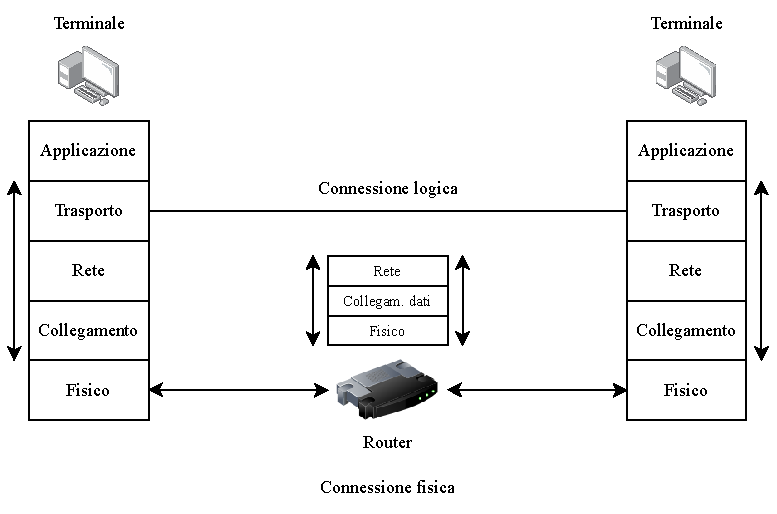
\includegraphics[width=\textwidth]{img/incapsulamento.pdf}
	\end{figure}

	La comunicazione avviene nel seguente modo:
	
	\begin{enumerate}
		\item Parte nel \textbf{\underline{livello di applicazione}} del host mittente il quale crea un \textbf{messaggio a livello di applicazione} (\emph{application-layer message}) concatenando informazioni aggiuntive, o meglio le informazioni di intestazione. Alla fine del processo di creazione, il messaggio viene passato al livello inferiore, quello di trasporto;
		
		\item A \textbf{\underline{livello di trasporto}} vengono aggiunte altre informazioni di intestazione. Le intestazioni di applicazione e trasporto formano il \textbf{segmento a livello di trasporto} (\emph{transport-layer segment}) che incapsula il messaggio a livello di applicazione. Infine, il livello di trasporto passa il messaggio al livello di rete;
		
		\item A \textbf{\underline{livello di rete}} vengono aggiunte informazioni come gli indirizzi dei sistemi periferici di sorgente e di destinazione. Facendo così viene creato un \textbf{datagramma a livello di rete} (\emph{network-layer datagram}). Infine, il messaggio viene passato al livello collegamento (\emph{link});
		
		\item A \textbf{\underline{livello di collegamento}} le informazioni aggiuntive creano un \textbf{frame a livello di collegamento} (\emph{link-layer frame});
		
		\item A \textbf{\underline{livello fisico}} vengono inviati i dati al router e qui termina l'incapsulamento.
	\end{enumerate}

	\noindent
	Per cui ad ogni livello, il pacchetto ha due tipi di campi: l’intestazione e \textbf{payload} (il carico utile trasportato). Il payload è tipicamente un pacchetto proveniente dal livello superiore.
\end{document}